\documentclass{article}%
\usepackage[T1]{fontenc}%
\usepackage[utf8]{inputenc}%
\usepackage{lmodern}%
\usepackage{textcomp}%
\usepackage{lastpage}%
\usepackage{geometry}%
\geometry{tmargin=2cm,lmargin=2cm}%
\usepackage{booktabs}%
\usepackage{graphicx}%
%
\title{Relatório de Dados {-} GDP e Obesidade}%
\author{Rafael Rodrigues, João Purificaçao}%
\date{\today}%
%
\begin{document}%
\normalsize%
\maketitle%
\section{Obesidade}%
\label{sec:Obesidade}%
\subsection{Estrutura}%
\label{subsec:Estrutura}%


\begin{table}[htbp]%
\centering%
\begin{tabular}{lllrrr}
\toprule
Sexes & Year & Country & Obesity\_Value (\%) & Obesity\_Min (\%) & Obesity\_Max (\%) \\
\midrule
Both sexes & 2016 & Afghanistan & 5.50 & 3.40 & 8.10 \\
Male & 2016 & Afghanistan & 3.20 & 1.30 & 6.40 \\
Female & 2016 & Afghanistan & 7.60 & 4.30 & 12.40 \\
Both sexes & 2015 & Afghanistan & 5.20 & 3.30 & 7.70 \\
Male & 2015 & Afghanistan & 3.00 & 1.30 & 6.00 \\
\bottomrule
\end{tabular}
%
\end{table}

%
\subsection{Comparação entre Homens e Mulheres:}%
\label{subsec:ComparaoentreHomenseMulheres}%


\begin{table}[htbp]%
\centering%
\begin{tabular}{lrr}
\toprule
 & Homens & Mulheres \\
\midrule
Média & 9.33 & 15.53 \\
Desvio Padrão & 8.98 & 11.32 \\
Mínimo & 0.10 & 0.20 \\
Máximo & 58.70 & 63.30 \\
\bottomrule
\end{tabular}
%
\caption{Relação entre os Sexos}%
\end{table}

%
\subsection{Percentuais na Ámerica do Norte:}%
\label{subsec:PercentuaisnamericadoNorte}%


\begin{table}[htbp]%
\centering%
\begin{tabular}{lr}
\toprule
 & Obesity\_Value (\%) \\
\midrule
Both Sexes & 28.03 \\
Males & 26.03 \\
Females & 29.77 \\
\bottomrule
\end{tabular}
%
\caption{Média do Países por Sexo}%
\end{table}

%
\newpage%
\subsection{Taxa de Aumento dos Índices de Obesidade:}%
\label{subsec:TaxadeAumentodosndicesdeObesidade}%
\subsubsection{Variação em 2010:}%
\label{ssubsec:Variaoem2010}%


\begin{table}[htbp]%
\centering%
\begin{tabular}{llr}
\toprule
Sexes & Country & Tax\_Obesity\_Value (\%) \\
\midrule
Both sexes & Sudan (former) & 1.40 \\
Male & Tuvalu & 1.00 \\
Male & Niue & 0.90 \\
Both sexes & Niue & 0.80 \\
Male & Micronesia (Federated States of) & 0.80 \\
Both sexes & Haiti & 0.80 \\
Female & Haiti & 0.80 \\
Female & Dominican Republic & 0.80 \\
Female & Costa Rica & 0.80 \\
\bottomrule
\end{tabular}
%
\caption{Maior Aumento de Taxa entre países em 2010}%
\end{table}

%


\begin{table}[htbp]%
\centering%
\begin{tabular}{llr}
\toprule
Sexes & Country & Tax\_Obesity\_Value (\%) \\
\midrule
Female & Japan & 0.10 \\
Female & Viet Nam & 0.10 \\
Both sexes & Democratic People's Republic of Korea & 0.10 \\
Both sexes & Japan & 0.10 \\
Both sexes & India & 0.10 \\
Male & Ethiopia & 0.00 \\
Male & Niger & 0.00 \\
Male & Eritrea & 0.00 \\
Female & Republic of Korea & 0.00 \\
\bottomrule
\end{tabular}
%
\caption{Menor Aumento de Taxa entre países em 2010}%
\end{table}

%
\subsubsection{Variação em 2016:}%
\label{ssubsec:Variaoem2016}%


\begin{table}[htbp]%
\centering%
\begin{tabular}{llr}
\toprule
Sexes & Country & Tax\_Obesity\_Value (\%) \\
\midrule
Both sexes & Haiti & 0.90 \\
Male & Niue & 0.90 \\
Male & Micronesia (Federated States of) & 0.80 \\
Male & Kiribati & 0.80 \\
Both sexes & Niue & 0.80 \\
Female & Haiti & 0.80 \\
Both sexes & Kiribati & 0.70 \\
Female & Saint Kitts and Nevis & 0.70 \\
Female & Vanuatu & 0.70 \\
\bottomrule
\end{tabular}
%
\caption{Maior Aumento de Taxa entre países em 2016}%
\end{table}

%


\begin{table}[htbp]%
\centering%
\begin{tabular}{llr}
\toprule
Sexes & Country & Tax\_Obesity\_Value (\%) \\
\midrule
Both sexes & Viet Nam & 0.10 \\
Male & Ethiopia & 0.10 \\
Male & Rwanda & 0.10 \\
Both sexes & Singapore & 0.10 \\
Male & Kenya & 0.10 \\
Female & Republic of Korea & 0.10 \\
Female & Israel & 0.10 \\
Both sexes & Sudan (former) & 0.00 \\
Female & Singapore & 0.00 \\
\bottomrule
\end{tabular}
%
\caption{Menor Aumento de Taxa entre países em 2016}%
\end{table}

%
\newpage%
\subsubsection{Variação no período completo:}%
\label{ssubsec:Variaonoperodocompleto}%


\begin{table}[htbp]%
\centering%
\begin{tabular}{lllr}
\toprule
Sexes & Year & Country & Tax\_Obesity\_Value (\%) \\
\midrule
Both sexes & 2015 & Sudan (former) & 2.80 \\
Both sexes & 1999 & Sudan (former) & 1.80 \\
Both sexes & 2007 & Sudan (former) & 1.50 \\
Female & 1990 & Tuvalu & 1.10 \\
Female & 1976 & Libya & 1.10 \\
Female & 1985 & Tuvalu & 1.00 \\
Male & 2004 & Cook Islands & 1.00 \\
Male & 1990 & Tuvalu & 1.00 \\
Male & 2003 & Cook Islands & 1.00 \\
\bottomrule
\end{tabular}
%
\caption{Maior Aumento de Taxa entre países}%
\end{table}

%


\begin{table}[htbp]%
\centering%
\begin{tabular}{lllr}
\toprule
Sexes & Year & Country & Tax\_Obesity\_Value (\%) \\
\midrule
Both sexes & 2002 & Sudan (former) & -1.30 \\
Both sexes & 2005 & Sudan (former) & -1.10 \\
Both sexes & 2009 & Sudan (former) & -1.00 \\
Male & 2015 & Sudan (former) & -0.60 \\
Male & 1977 & Somalia & 0.00 \\
Male & 1976 & Afghanistan & 0.00 \\
Female & 1978 & Viet Nam & 0.00 \\
Female & 2009 & Singapore & 0.00 \\
Female & 1976 & Afghanistan & 0.00 \\
\bottomrule
\end{tabular}
%
\caption{Menor Aumento de Taxa entre países}%
\end{table}

%
\newpage%
\subsection{Apanhando sobre o Brasil:}%
\label{subsec:ApanhandosobreoBrasil}%
\subsubsection{Variação em 2010:}%
\label{ssubsec:Variaoem2010}%


\begin{table}[htbp]%
\centering%
\begin{tabular}{lr}
\toprule
 & Obesity\_Value (\%) \\
\midrule
Both Sexes & 28.03 \\
Males & 26.03 \\
Females & 29.77 \\
\bottomrule
\end{tabular}
%
\caption{Média do Países por Sexo}%
\end{table}

%
\newpage%
\section{GDP}%
\label{sec:GDP}%
\subsection{Dados}%
\label{subsec:Dados}%


\begin{figure}[htbp]%
\centering%
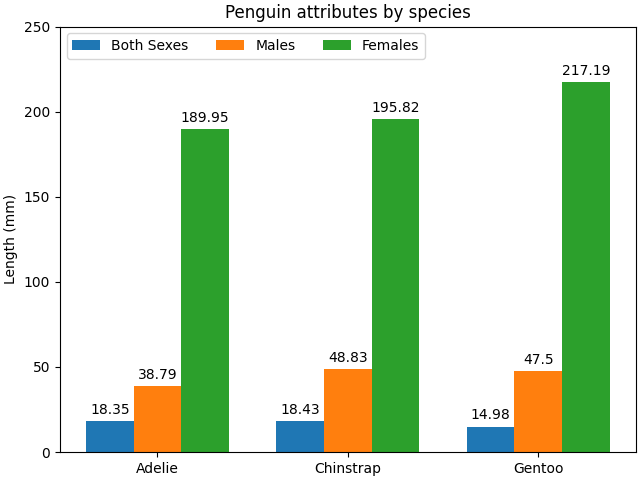
\includegraphics[width=300px]{img/foo.png}%
\caption{Look it's on its back}%
\end{figure}

%
\end{document}